\documentclass{article}

\usepackage[french]{babel}
\usepackage[utf8]{inputenc}
\usepackage{amsmath}
\usepackage{hyperref}
\usepackage{graphicx}
\usepackage{subcaption}
\usepackage{listings}
\usepackage{algorithm}
\usepackage{algpseudocode}

%%%%%%%%%%%%% Aspect of links %%%%%%%%%%%%
\hypersetup{
	colorlinks=true,
	linkcolor=magenta,
	citecolor=blue,
	pdfborder={0 0 0}
}

%%%%%%%%%%%%%%%% Lengths %%%%%%%%%%%%%%%%%
\setlength{\textwidth}{15.5cm}
\setlength{\evensidemargin}{0.5cm}
\setlength{\oddsidemargin}{0.5cm}

%%%%%%%%%%%%%%%% Variables %%%%%%%%%%%%%%%%
\def\projet{1}
\def\titre{\textbf{Compression d’image à travers la factorisation SVD}}
\def\groupe{3}
\def\equipe{4}
\def\responsible{Camille LAMBLOT}
\def\secretary{Soufiane SBAI}
\def\others{Mohamed KRAIMY, Ilian HAMMANI}

\begin{document}

%%%%%%%%%%%%%%%% Header %%%%%%%%%%%%%%%%
\noindent\begin{minipage}{0.98\textwidth}
  \vskip 0mm
  \noindent
  { \begin{tabular}{p{7.5cm}}
  	{\bfseries \sffamily}
  	{\itshape \titre}
	\end{tabular}}
  \hfill
  \fbox{\begin{tabular}{l}
  	{~\hfill \bfseries \sffamily Groupe \groupe\ - Equipe \equipe
    	\hfill~} \\[2mm]
  	Responsable : \responsible \\
  	Secrétaire : \secretary \\
  	Codeurs : \others
	\end{tabular}}
  \vskip 4mm ~

  ~~~\parbox{0.95\textwidth}{\textit{Résumé~:} \sffamily Ce projet a pour objectif d'implémenter un algorithme de compression d'images basé sur la factorisation en valeurs singulières (SVD).  
Dans un premier temps, nous étudierons les transformations de Householder, depuis leur construction jusqu'à leur utilisation dans la factorisation SVD.  
Ensuite, nous implémenterons un algorithme de réduction d'une matrice rectangulaire en forme bidiagonale.  
Puis, nous développerons et optimiserons un algorithme de transformations QR, étape clé du calcul de la SVD.  
Enfin, nous appliquerons cette méthode à la compression d'une image et analyserons l'\'efficacit\'e de cette compression.
  }
  \vskip 1mm ~
\end{minipage}

%%%%%%%%%%%%%%%% Main part %%%%%%%%%%%%%%%%

\renewcommand{\contentsname}{Table des matières}
{\hypersetup{linkcolor=black}\tableofcontents}

\section{Transformation de Householder}
\subsection{Construction de la matrice de Householder}

La matrice de Householder \( H \) est définie par la relation :
\[
H = I - 2 \times N N^T
\]
où \( I \) est la matrice identité et \( N \) est un vecteur unitaire normal à l'hyperplan passant par \( U \) et \( V \). Ce vecteur \( N \) est calculé comme :
\[
N = \frac{U - V}{\|U - V\|}
\]
Ce calcul garantit que \( N \) est un vecteur de norme 1, et que la transformation de Householder agit comme une réflexion qui envoie \( U \) sur \( V \). L'objectif de cette transformation est de rendre la matrice plus simple à manipuler, notamment en réduisant les matrices à des formes plus diagonales ou bidiagonales, facilitant ainsi les calculs dans des algorithmes comme la décomposition SVD.

\subsection{Application de la transformation de Householder}

Dans ce projet, nous avons utilisé la transformation de Householder pour simplifier la réduction des matrices en l'appliquant directement sur chaque colonne. Plutôt que de calculer et stocker la matrice complète \( H \) de taille \( n \times n \), nous conservons uniquement le vecteur \( U \), ce qui permet un calcul plus efficace de \( H(U) \) en \( O(n) \). Cette approche améliore à la fois la complexité spatiale et temporelle.\\
Nous avons mis en place plusieurs fonctions pour effectuer cette transformation :

\begin{itemize}
    \item \textbf{projection(U, V)} : Calcule le vecteur normal \( N \) de la transformation de Householder, défini ci-dessus.
    Cela permet de construire la réflexion sans avoir à manipuler directement la matrice \( H \).

    \item \textbf{householdervector(N, X)} : Applique la transformation de Householder sur un vecteur \( X \) en évitant de stocker \( H \). Elle est définie par :
    \[
    H(X) = X - 2 <N,X> N
    \]
    Cette approche optimise la complexité en évitant le stockage de la matrice H de taille n x n.

    \item \textbf{householder\_on\_matrix(U, V, M)} : Applique la transformation de Householder à chaque colonne d'une matrice \( M \). Plutôt que de multiplier explicitement par \( H \), nous appliquons la transformation individuellement à chaque colonne, ce qui réduit le coût.
\end{itemize}

\subsection{Analyse de la complexité}

L'application de Householder à un vecteur nécessite un produit scalaire, soit une complexité de \( O(n) \). En l'appliquant successivement aux \( m \) colonnes d'une matrice \( n \times m \), la complexité totale est \( O(nm) \), bien plus optimale que \( O(n^2 m) \) pour un produit matrice-matrice classique. Cette optimisation est particulièrement bénéfique pour les matrices rectangulaires où \( m \ll n \).

\section{Mise sous forme bidiagonale}
\subsection{Algorithme de Réduction Bidiagonale}

L'algorithme de réduction bidiagonale consiste en une double application de transformations de Householder :

\begin{enumerate}
    \item \textbf{Réduction des colonnes} : À chaque étape \( k \), on applique une transformation de Householder \( H_k \) pour annuler les éléments sous la diagonale dans la colonne \( k \).
    \item \textbf{Réduction des lignes} : Ensuite, une autre transformation de Householder \( G_k \) est appliquée pour annuler les éléments à droite de la première sous-diagonale de la ligne \( k \).
    \item \textbf{Mise à jour des matrices accumulées} : Les matrices orthogonales \( U \) et \( V \) sont mises à jour à chaque étape.

    \item \textbf{Invariant} : A chaque itération, on vérifie que le produit \[ A = Q_{left} * B * Q_{right}  \] est bien conservé.
\end{enumerate}

La procédure est répétée pour chaque colonne et ligne jusqu'à obtenir une matrice strictement bidiagonale.

\subsection{Complexité de l'Algorithme de Bidiagonalisation}

L'algorithme de bidiagonalisation utilise des transformations de Householder pour chaque ligne et colonne. À chaque étape, les opérations principales (calcul de la norme et multiplication matricielle) ont une complexité de \( O(n) \) pour les lignes et \( O(m) \) pour les colonnes. L'algorithme s'exécute sur \( \min(n, m) \) étapes, ce qui donne une complexité temporelle totale de \( O(n m^2) \).

En termes d'espace, l'algorithme nécessite de stocker la matrice \( A \), les matrices orthogonales \( Q_{\text{left}} \) et \( Q_{\text{right}} \), et la matrice bidiagonale \( BD \), ce qui donne une complexité spatiale de \( O(n^2 + m^2) \).

\section{Optimisation de la décomposition QR pour les matrices bidiagonales}

Dans cette section, nous présentons une version optimisée de l'algorithme de décomposition QR pour les matrices bidiagonales. L'idée principale est de tirer parti de la structure particulière de ces matrices, ce qui permet de réduire le coût computationnel par rapport à la décomposition QR classique.

\subsection{Description de l'Algorithme Optimisé}

L'algorithme optimise la décomposition QR en manipulant directement les éléments non nuls de la matrice bidiagonale. Plutôt que de traiter une matrice complète, l'algorithme travaille sur des blocs de taille \( 2 \times 2 \) en réduisant les matrices à une taille minimale, ce qui permet une meilleure gestion des ressources et des calculs.

Dans le fichier \texttt{qr\_algorithm.py}, l'algorithme manipule les éléments de la matrice \( R \) en utilisant la transformation de Householder. Plutôt que de travailler avec une matrice de grande taille comme
\[
X = \begin{bmatrix} R_{i,i} & R_{i+1,i} & 0 & 0 & 0 & 0 & \dots \end{bmatrix},
\]
Il réduit cette matrice à un bloc plus petit :
\[
X = \begin{bmatrix} R_{i,i} & R_{i+1,i} \end{bmatrix}, \quad Y = \begin{bmatrix} \alpha & 0 \end{bmatrix}, \quad \alpha = \left\lVert X \right\rVert
\]
ce qui permet de manipuler des matrices \( 2 \times 2 \), plus efficaces à traiter.


La matrice de Householder \( H \) est alors appliquée de manière sélective pour préserver la structure bidiagonale de \( R \), en utilisant une matrice de transformation de la forme suivante :
\[
\begin{bmatrix}
I & 0 & 0 \\
0 & H & 0 \\
0 & 0 & I
\end{bmatrix}
\]
où \( I \) est la matrice identité et \( H \) est la matrice de Householder appliquée sur les colonnes de \( R \) et les lignes de \( Q \).




Ainsi, cette approche permet de réduire les calculs tout en maintenant la structure de la matrice et en optimisant les performances de l'algorithme. La complexité de cette méthode est de \(O(n^2)\), ce qui correspond au coût de l'application de la transformation de Householder sur les lignes et les colonnes de \(R\) et \(Q\). Cette optimisation permet d'éviter de manipuler des matrices de grande taille, ce qui améliore l'efficacité de l'algorithme tout en préservant la structure bidiagonale.


\section{Analyse de la convergence de la matrice \( S \)}




\subsection{Convergence de la matrice \( S \)}

Afin de visualiser la convergence de la matrice \( S \), nous avons d'abord utilisé une version préliminaire de l'algorithme avec la fonction \texttt{numpy.linalg.qr}, puis une version optimisée avec \texttt{qr\_optimise}. Nous présentons ci-dessous les courbes de convergence de la matrice \( S \) vers une matrice diagonale pour ces deux méthodes.


\begin{figure}[H]
\centering
\begin{minipage}{0.45\textwidth}
    \centering
    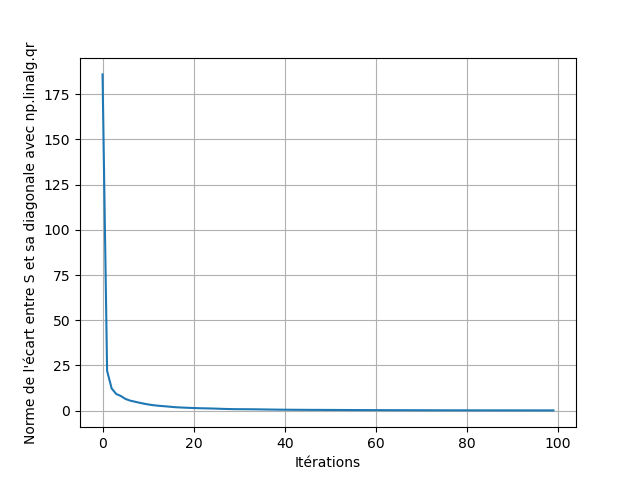
\includegraphics[width=\textwidth]{np.linalg.qr.png}
    \caption{Convergence de la matrice \( S \) avec \texttt{np.linalg.qr}}
    \label{fig:convergence_np_qr}
\end{minipage} \hfill
\begin{minipage}{0.45\textwidth}
    \centering
    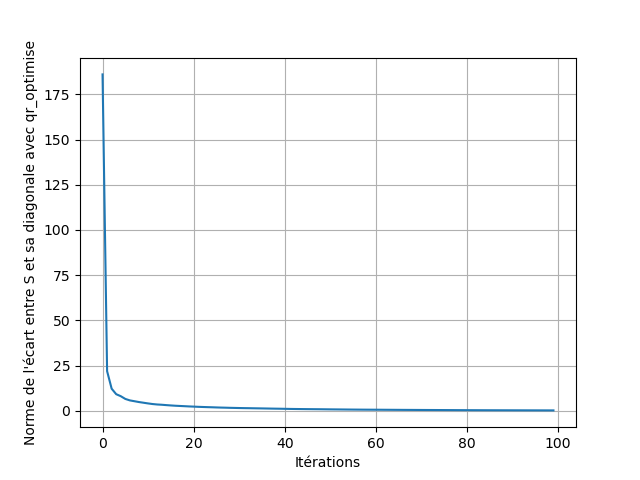
\includegraphics[width=\textwidth]{qr_optimise.png}
    \caption{Convergence de la matrice \( S \) avec \texttt{qr\_optimise}}
    \label{fig:convergence_qr_optimise}
\end{minipage}
\end{figure}

Les graphiques \ref{fig:convergence_np_qr} et \ref{fig:convergence_qr_optimise} illustrent la convergence de la matrice \( S \) vers une matrice diagonale. Pour cette analyse, nous avons utilisé l'image d'entrée \texttt{p3\_takeoff\_base.png}, dont nous avons extrait la composante rouge sous forme de matrice \( \texttt{img\_r} \).  

Nous avons ensuite appliqué notre algorithme de décomposition en valeurs singulières (SVD) à cette matrice \( \texttt{img\_r} \), en comparant deux méthodes : \texttt{np.linalg.qr} et \texttt{qr\_optimise}. Pour évaluer la convergence de \( S \), nous avons tracé la norme de l'écart entre \( S \) et sa diagonale en fonction du nombre d'itérations.  

Comme on peut l'observer, la matrice \( S \) converge progressivement vers une forme diagonale dans les deux cas, montrant ainsi le bon fonctionnement des deux méthodes.  

\subsection{Analyse de l'invariant dans l'algorithme de décomposition SVD}

La transformation QR d'une matrice bidiagonale produit une matrice bidiagonale. À chaque itération de notre algorithme, nous effectuons les opérations suivantes :
\begin{itemize}
    \item \( S^T = Q_1 \times R_1 \), où \( R_1 \) est une matrice bidiagonale supérieure.
    \item \( R_1^T = Q_2 \times R_2 \), où \( R_2 \) reste également bidiagonale.
\end{itemize}

La structure bidiagonale est ainsi préservée car la décomposition QR d'une matrice bidiagonale donne une matrice bidiagonale. Cela garantit que \( S \), \( R_1 \), et \( R_2 \) conservent cette forme tout au long de l'algorithme.

Nous vérifions également l'invariant suivant à chaque étape de l'algorithme de décomposition \( U \times S \times V = BD \), où \( BD \) est la matrice obtenue par la méthode de bidiagonalisation.


\section{Application à la compression d'image}



\subsection{Gain de Place et Rang Maximal}
Le gain de place d'une matrice \( A \) après compression au rang \( r \) peut être défini par la différence entre la taille originale et la taille compressée de la matrice. Si \( A \) est une matrice de taille \( n \times m \), la taille compressée après compression au rang \( r \) est donnée par :

\[
\text{Taille compressée} = n \times r + r \times m + r^2
\]

La taille originale est simplement \( n \times m \), et le gain de place est donc :

\[
\text{Gain de place} = n \times m - (n \times r + r \times m + r^2)
\]

En outre, il existe un rang maximal \( r_{\text{max}} \) au-delà duquel la compression n'est plus avantageuse. Ce rang est donné par la solution de l'inégalité quadratique suivante (car nous voulons que la taille compressée soit supérieure à la taille originale):

\[
r^2 + r(n + m) - n \times m \geq 0
\]
La solution de cette inégalité est :

\[
r_{\text{max}} = \frac{-(n + m) + \sqrt{(n + m)^2 + 4 \times n \times m}}{2}
\]

Ainsi, \( r_{\text{max}} \) est le plus grand entier \( r \) pour lequel cette condition est satisfaite.

\subsection{Efficacité de la Compression}
Nous avons analysé l'efficacité de la compression en comparant la distance entre la matrice originale et la matrice compressée pour les différents rangs suivants [5, 50, 100, 130, 150, 200]. La distance entre ces matrices a été mesurée à l'aide de la norme Euclidienne, ce qui permet de quantifier l'écart entre l'image originale et l'image compressée. Pour cette analyse, nous avons utilisé la matrice de la composante rouge de l'image \texttt{p3\_takeoff\_base.png}.

\begin{figure}[h!]
\centering
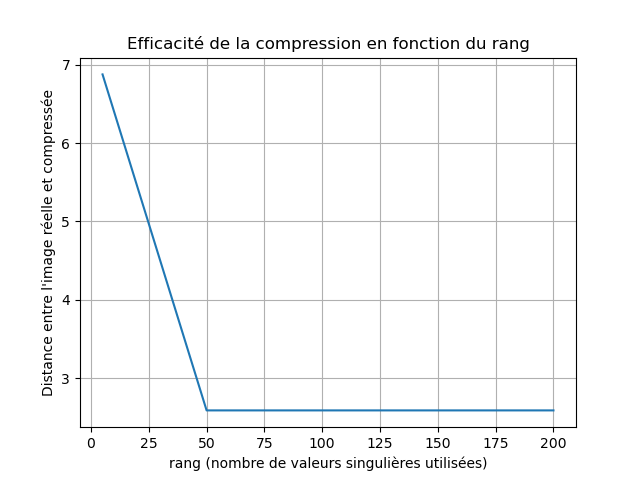
\includegraphics[width=0.6\textwidth]{efficacite_compression.png}
\caption{Évolution de l'efficacité de la compression en fonction du rang}
\label{fig:efficacite_compression}
\end{figure}

La figure \ref{fig:efficacite_compression} montre l'évolution de cette distance en fonction du rang de compression. À mesure que le rang augmente, la distance diminue. Cela est bien, car on annule moins de termes, permettant ainsi une meilleure préservation des informations dans la matrice compressée.


\subsection{Compression de l'image \texttt{p3\_takeoff\_base.png}}

\begin{figure}[h!]
\centering
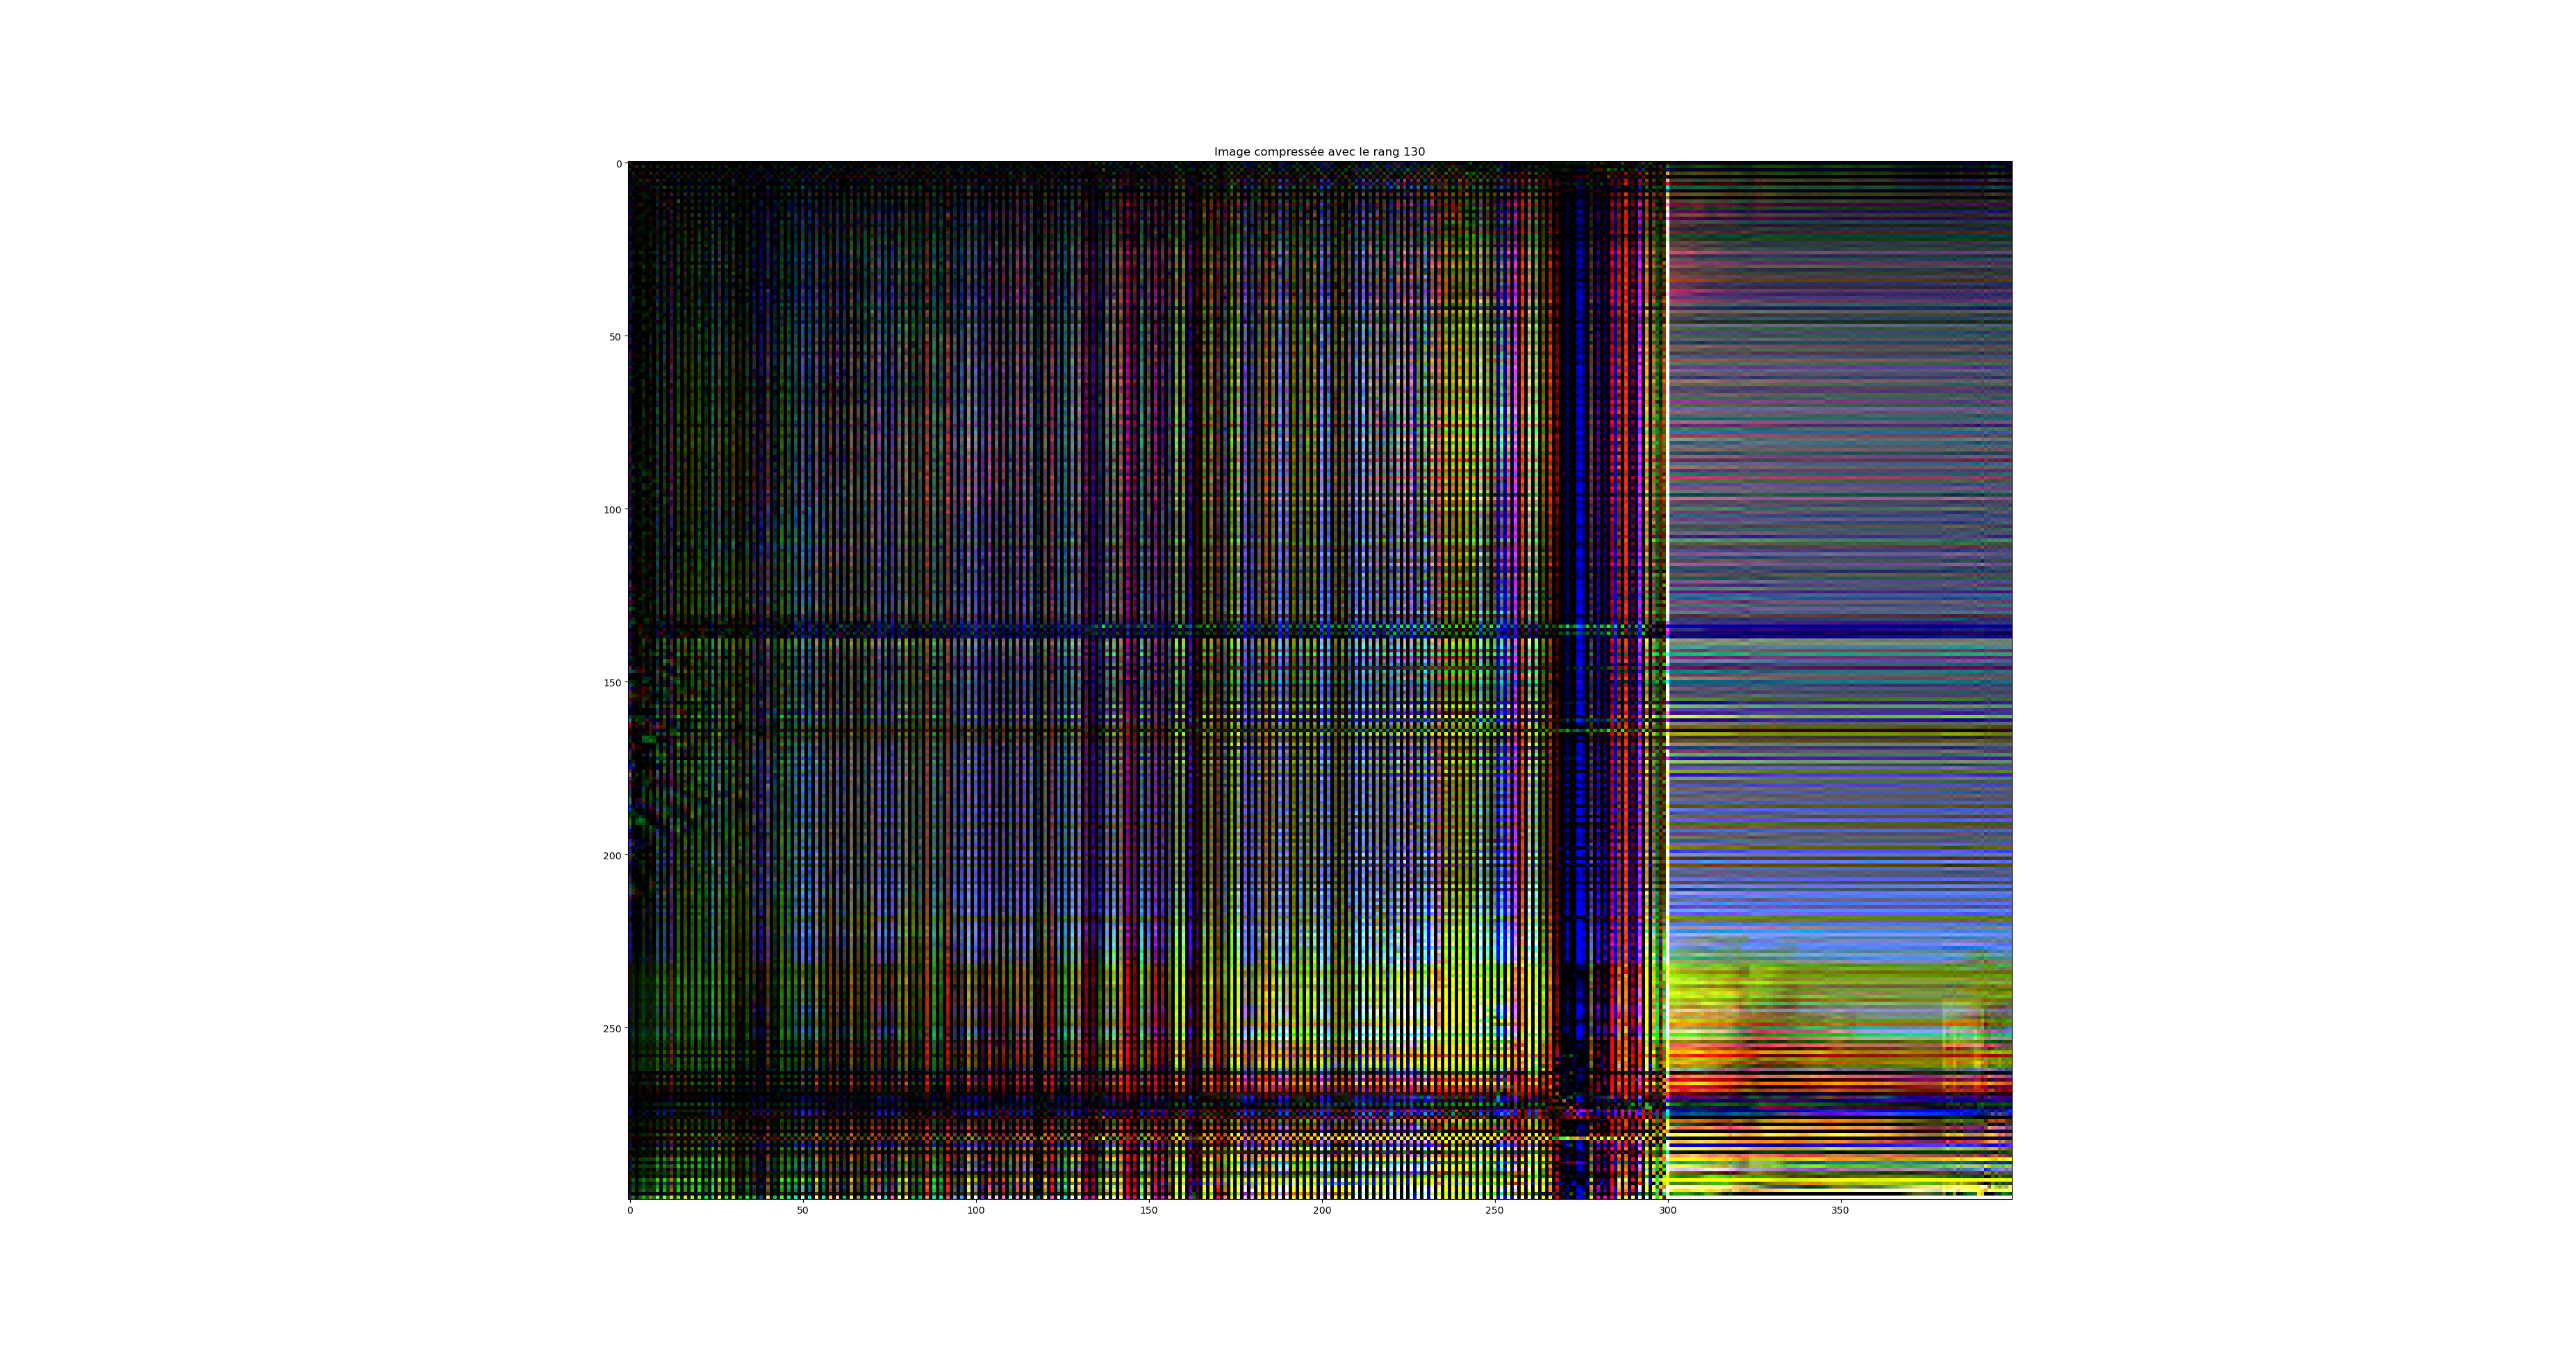
\includegraphics[width=0.7\textwidth]{compression 130.png}
\caption{Compression de \texttt{p3\_takeoff\_base.png} au rang 130}
\end{figure}
Nous avons tenté de compresser l'image \texttt{p3\_takeoff\_base.png} au rang 130. Cependant, comme on peut le voir sur l'image ci-dessus, le résultat de la compression n'est pas celui attendu. Bien que tout le code fonctionne correctement et que toutes les étapes aient été vérifiées, la compression ne semble pas avoir bien fonctionné. Nous avons exploré plusieurs approches, mais n'avons pas encore réussi à obtenir le résultat souhaité. Nous sollicitons donc votre aide pour comprendre ce qui pourrait poser problème.


\end{document}
